\documentclass[12pt, bachelor, substylefile = algo_title.rtx]{disser}

\usepackage[a4paper,
            left=1.5cm, right=1.5cm,
            top=2cm, bottom=2cm,
	 headsep=1cm, footskip=1cm]{geometry}
\usepackage[T2A]{fontenc}
\usepackage[utf8]{inputenc}
\usepackage[english]{babel}
\usepackage{amsmath, amsthm}
\usepackage{hyperref}
\usepackage{amsfonts}
%\usepackage{indentfirst}
\usepackage{xcite}
\usepackage{xr}
\usepackage{outlines}
\usepackage{mathtools}
\usepackage{subcaption}
\usepackage[table]{xcolor}
%\usepackage{newtxtext,newtxmath}
\usepackage[final]{pdfpages}


\DeclarePairedDelimiter\ceil{\lceil}{\rceil}
\DeclarePairedDelimiter\floor{\lfloor}{\rfloor}
\newcommand{\Hyp}{\ensuremath{\mathbb{H}}}
\newcommand{\Pb}{\mathcal{P}}
\newcommand{\ME}{\mathbb{E}}
\newcommand{\med}{\mathbb{M}}
\newcommand{\Proba}{\mathbb{P}}
\newcommand{\VAR}{\mathbb{D}}
\newcommand{\varD}{\mathbf{D}}
\newcommand{\eps}{\varepsilon}
\newcommand{\varZ}{\mathbf{Z}}
\newcommand{\varV}{\mathbf{V}}
\newcommand{\varW}{\mathbf{W}}
\newcommand{\varY}{\mathbf{Y}}
\newcommand{\varX}{\mathbf{X}}
\newcommand{\varR}{\mathbf{R}}
\newcommand{\varS}{\mathbf{S}}
\newcommand{\varU}{\mathbf{U}}
\newcommand{\ind}{\mathbb{I}}
\newcommand{\Real}{\mathbb{R}}
\newcommand{\Sample}{\varV_1,\varV_2,\dots,\varV_m}
\newcommand{\Samplex}{\varX_1,\varX_2,\dots,\varX_n}
\DeclareMathOperator{\sign}{sign}

\newcommand{\specialcell}[2][c]{%
  \begin{tabular}[#1]{@{}c@{}}#2\end{tabular}}

\theoremstyle{definition}
\newtheorem{theorem}{Theorem}
\newtheorem{definition}{Definition}
\newtheorem{assumption}{Assumption}
\newtheorem{lemma}{Lemma}
\newtheorem{example}{Example}
\newtheorem{proposition}{Proposition}
\newtheorem{conseq}{Consequence}

\setcounter{tocdepth}{2}


\begin{document}

\institution{FEDERAL STATE AUTONOMOUS EDUCATIONAL INSTITUTION\\
OF HIGHER EDUCATION\\
ITMO UNIVERSITY
}
\title{Report on learning practice \#3}


\topic{\normalfont\scshape %
Sampling of multivariate random variables}
\author{Dmitry Grigorev,\\ Eugenia Khomenko,\\ Efim Podkovirkin,\\ Arina Syrchenko}

\city{St. Petersburg}
\date{2022}

\maketitle

\tableofcontents

\section{Data description}

Let $D$ be the modified dataset on Narvik roads. The features here are:

\begin{outline}
\1lat\_ — latitude
\1 lon\_ — longitude
\1 State\_ — word description of road state (1: 'dry', 2: 'moist', 3: 'wet', 4: 'icy', 5: 'snowy', 6: 'slushy')
\1 Ta\_mean,Ta\_min,Ta\_max — atmosphere temperature
\1 Tsurf\_mean,Tsurf\_min,Tsurf\_max — surface temperature
\1 Water\_mean,Water\_min,Water\_max — water layerw width (0 -- 3 $mm$)
\1 Speed\_mean,Speed\_min,Speed\_max — wind speed (in knots, $5\ knots \approx 9.3\ km/h$)
\1 Height\_mean,Height\_min,Height\_max — height of location above mean sea level
\1 Tdew\_mean,Tdew\_min,Tdew\_max — dew point ($Celsius$)
\1 Friction\_mean,Friction\_min,Friction\_max — friction value ( 0 -- 1, 0 means no friction)
\1 Date,Time, date\_time, FullDate — time and date
\1 Direction\_min,Direction\_max — wind direction ($degrees$)
\1 ClosestCity, location
\1 maxtempC,mintempC — day maximum and minimum of temperature ($Celsius$)
\1 totalSnow\_cm — total snowfall ($cm$)
\1 sunHour — passed sun energy in $Sun-Hours$ (A $Sun-Hour$ is "1000 watts of energy shining on 1 square meter of surface for 1 hour")
\1 uvIndex — ultraviolet index
\1 moon\_illumination — moon phase ($percents$)
\1 moonrise — time of Moon rise
\1 moonset — time of Moon set
\1 sunrise — time of Sun rise
\1 sunset — time of Sun set
\1 DewPointC — hourly dew point measurement ($Celsius$)
\1 FeelsLikeC — hourly Feels-like temperature ($Celsius$)
\1 HeatIndexC — hourly heat index ($Celsius$)
\1 WindChillC — hourly wind-chill index ($Celcius$) 
\1 WindGustKmph — hourly wind gust measure ($km/h$)
\1 cloudcover — hourly cloud cover index ($percents$)
\1 humidity — hourly humidity ($percents$)
\1 precipMM — hourly precipitation ($mm$)
\1 pressure — hourly atmosphere pressure ($mbar$)
\1 tempC — hourly atmosphere temperature ($Celsius$)
\1 visibility — hourly visibility (0--10, 0 means poor visibility)
\1 winddirDegree — hourly wind direction ($degrees$)
\1 windspeedKmph — hourly wind speed ($km/h$)
\end{outline}


\begin{figure}[!h]
\centering
   \begin{minipage}{0.7\textwidth}
     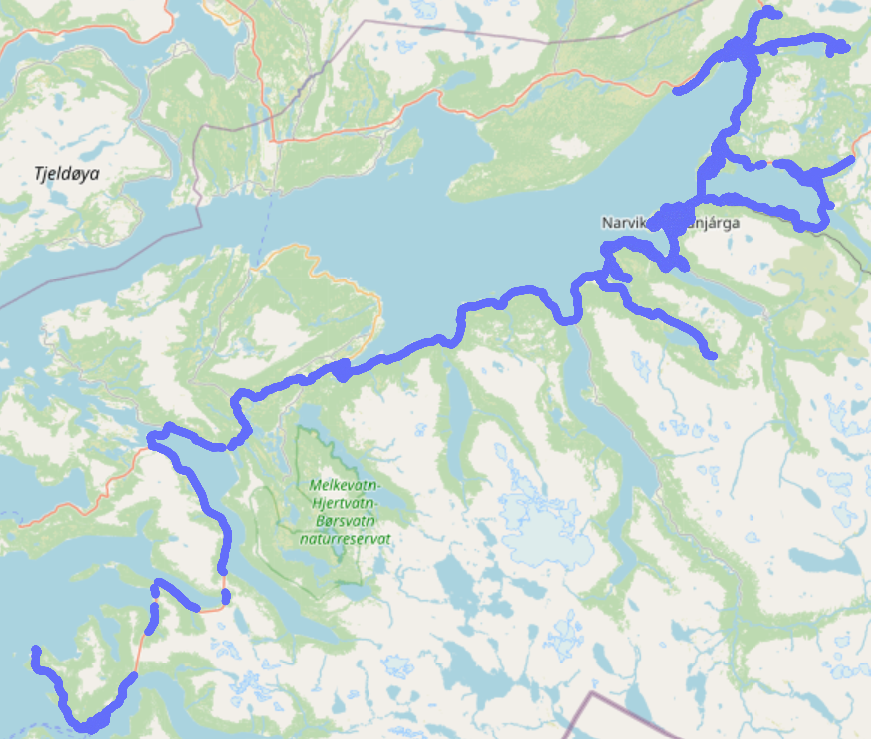
\includegraphics[width=\linewidth]{geography}
   \end{minipage}
\caption{Geography of the data}
\label{fig: 1}
\end{figure}

\section{Substantiation of chosen sample}
In this lab work Friction\_mean, windspeedKmph and FeelsLikeC are chosen as targets and the predictors  are humidity, State\_, pressure, Height\_mean, totalSnow\_cm, Water\_mean, moon\_illumination. Further we test the significance of dependence between chosen targets and predictors. We have chosen 1000 observations as a subsample.

\section{Additional research on appropriate distribution}
As a result of Lab \#1 it was obtained that
\begin{outline}
\1 the most appropriate distribution for FeelsLikeC is normal with $\mu \approx -8.867$ and $\sigma \approx 5.874$ (it minimizes least squares and maximizes log-likelihood);
\1 the most appropriate distribution for windspeedKmph is Cauchy's with $loc \approx 11.637$ and $scale \approx 2.830$ (it minimizes least squares and maximizes log-likelihood).
\end{outline} 

Feature Friction\_mean was under focus in Lab \#2 where linear regression model for this feature has been built. Its distribution is bimodal (see fig. \ref{fig: 2}) so any simple continuous distribution would not fit here for estimation. As an example, it is proposed to find   the mixture of two normal distributions $\Pb = (1-\alpha) N(\mu_1, \sigma^2_1) + \alpha N(\mu_2, \sigma^2_2)$. 

\begin{figure}[!h]
\centering
   \begin{minipage}{0.7\textwidth}
     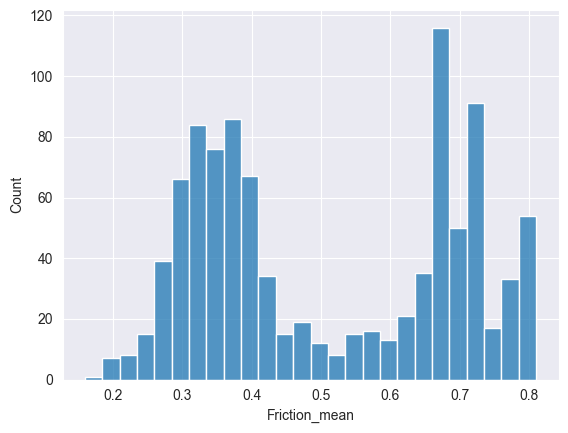
\includegraphics[width=\linewidth]{friction}
   \end{minipage}
\caption{Histogram of Friction\_mean}
\label{fig: 2}
\end{figure}

To find the unknown parameters we have applied EM algorithm which we implemented for the two components normal distribution mixture separation (see \cite{repogithub}). As a result, we obtained the following parameters:
\begin{align*}
\alpha & \approx 0.463,\\
\mu_1 & \approx 0.353,\\
\sigma_1 & \approx 0.065,\\
\mu_2 & \approx 0.694,\\
\sigma_2 & \approx 0.063,\\
\end{align*}
and the corresponding distribution is illustrated in figure \ref{fig: 3}.

\begin{figure}[!h]
\centering
   \begin{minipage}{0.7\textwidth}
     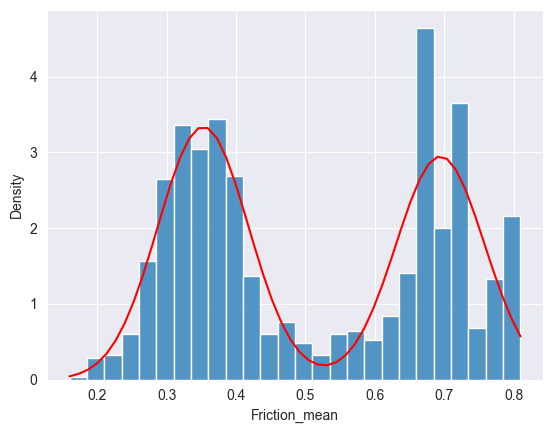
\includegraphics[width=\linewidth]{estim}
   \end{minipage}
\caption{The found mixture of two gaussians which fits the data of Friction\_mean}
\label{fig: 3}
\end{figure}

As one can see from the figure \ref{fig: 3}, the obtained mixture fits the data quite well. The QQ-plot of data vs the mixture in picture \ref{fig: 4} also allows us to conclude the same. However, Kolmogorov-Smirnov test under significance level $\widetilde{\alpha} = 0.05$ with p-value$ \approx 0.009$ rejects the hypothesis that our sample came from the distribution described by the mixture. That is why we do not expect that a synthesized sample will follow the same distribution as Friction\_mean.

\begin{figure}[!h]
\centering
   \begin{minipage}{0.7\textwidth}
     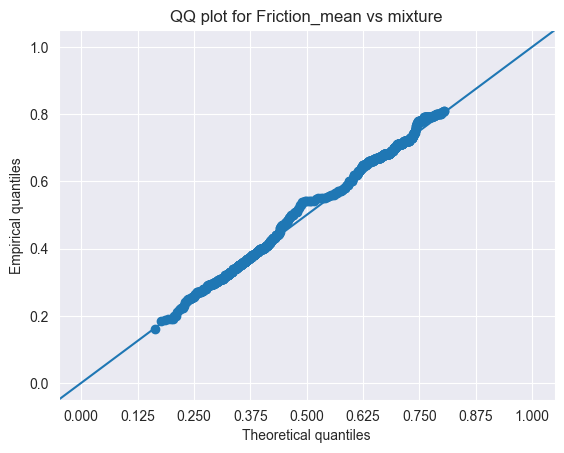
\includegraphics[width=\linewidth]{qqmix}
   \end{minipage}
\caption{QQ-plot for Friction\_mean versus the found mixture}
\label{fig: 4}
\end{figure}

\section{Sampling of chosen target variables using univariate parametric distributions
(from practice \#1) with 2 different sampling methods}
\subsection*{Friction\_mean}
To generate a sample for Friction\_mean by means of the fitted distribution, we used Box-Muller algorithm which generates normal distribution given a mixture component and the mixture component number probability is determined by $\alpha$, and acceptance-rejection sampling (ARS) with bins which inner distribution is uniform across a bin and probability is proportional to the bin area.

The idea behind Box-Muller algorithm is as follows: given i.i.d $\alpha_1, \alpha_2 \sim U(0,1)$, the variables
\[ \xi_1 = \sqrt{-2\ln (\alpha_1)}\sin(2\pi \alpha_2),  \xi_2 = \sqrt{-2\ln (\alpha_1)}\cos(2\pi \alpha_2) \]
are i.i.d. and $\xi_i \sim N(0, 1)$. The number of mixture component is a random variable with values 1 and 2 and probabilities $(1-\alpha)$ and $\alpha$ correspondingly. To obtain $\xi \sim N(\mu, \sigma^2)$ from $\eta \sim N(0, 1)$ one has to perform linear transformation: $\xi \gets \sigma \eta + \mu$. 

As soon as a sample of 1000 elements was obtained from the found distribution by the Box-Muller algorithm, two sample Kolmogorov-Smirnov test was performed under significance level $\widetilde{\alpha} = 0.05$. Its p-value$ \approx 0.164$ so there is no evidence to reject the hypothesis that the synthesized sample came from the same distribution as our sample. Two figures in fig. \ref{fig: 5} demonstrate to what extent the generated sample is similar to the theoretical distribution and the empirical distribution of Friction\_mean.

\begin{figure}[!h]
   \begin{minipage}{.48\textwidth}
     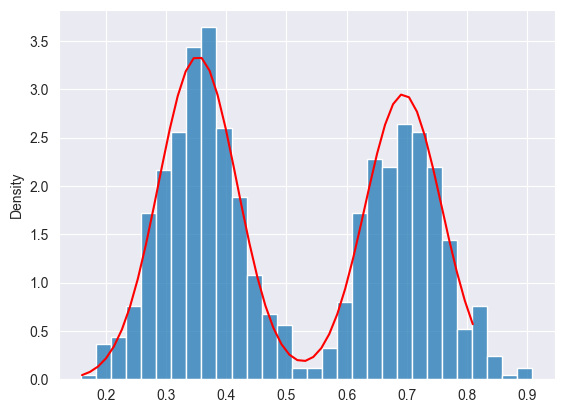
\includegraphics[width=\linewidth]{eta0}
   \end{minipage} \hfill
\begin{minipage}{.48\textwidth}
     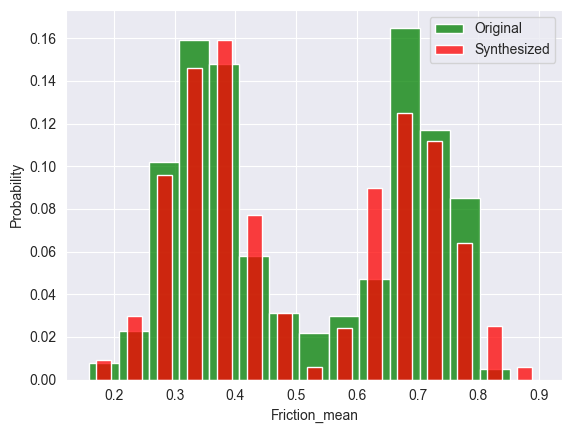
\includegraphics[width=\linewidth]{eta1}
   \end{minipage}
\caption{The histogram of the generated sample vs the mixture's density and the histogram of observed Friction\_mean}
\label{fig: 5}
\end{figure}

As for the second algorithm of sampling, we performed partition of the range of Friction\_mean variable into 6 bins and built piece-wise constant majorant depicted in figure \ref{fig: 6}. It is worth mentioning that we restricted the mixture on the Friction\_mean range interval with the corresponding normalization so that the integral of the density is equal to 1. Further we use this majorant in ARS to make sampling efficient. Each bin determines its own rectangle in which ARS is performed and its own sampling distribution which is uniform by our choice. The sampling scheme is presented in \cite{Marholm20}.



\begin{figure}[!h]
\centering
   \begin{minipage}{0.7\textwidth}
     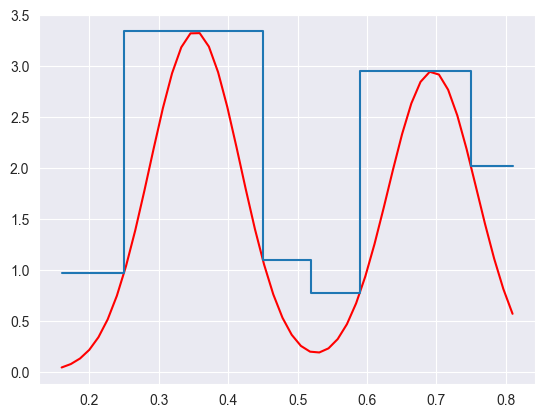
\includegraphics[width=\linewidth]{major}
   \end{minipage}
\caption{The majorant of the mixture's density}
\label{fig: 5}
\end{figure}

As a result of sampling by the aforementioned method, we obtained a sample of 1000 observations and two sample Kolmogorov-Smirnov test under significance level $\widetilde{\alpha} = 0.05$ executed $p-value \approx 0.006$ rejects the hypothesis that the real data sample and the synthesized sample came from the same distribution. 
Two figures in fig. \ref{fig: 6} demonstrate to what extent the generated sample is similar to the theoretical distribution and the empirical distribution of Friction\_mean.

\begin{figure}[!h]
   \begin{minipage}{.48\textwidth}
     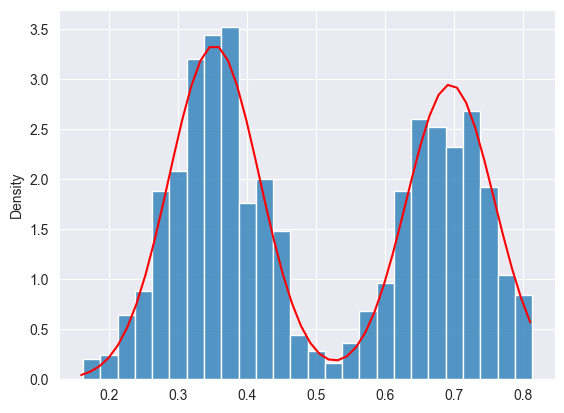
\includegraphics[width=\linewidth]{ars0}
   \end{minipage} \hfill
\begin{minipage}{.48\textwidth}
     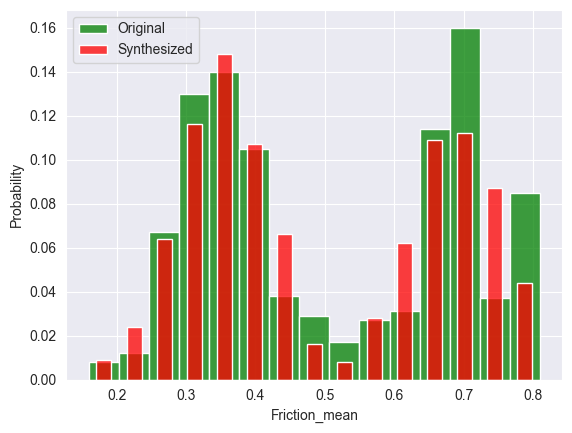
\includegraphics[width=\linewidth]{ars1}
   \end{minipage}
\caption{The histogram of the ARS-generated sample vs the mixture's density and the histogram of observed Friction\_mean}
\label{fig: 6}
\end{figure}

\subsection*{FeelsLikeC}
In Lab \#1 it was obtained that the appropriate distribution for FeelsLikeC is normal $N(\mu, \sigma^2)$ with $\mu \approx -8.867,\ \sigma \approx 5.873$. To simulate the normal distribution we used Box-Muller algorithm and ARS with sampling from Laplace distribution.

As soon as a sample of 1000 elements was obtained from the found distribution by the Box-Muller algorithm, two sample Kolmogorov-Smirnov test was performed under significance level $\widetilde{\alpha} = 0.05$. Its p-value$ \approx 0.00028$ so it rejects the hypothesis that the synthesized sample came from the same distribution as our sample. Two figures in fig. \ref{fig: 7} demonstrate to what extent the generated sample is similar to the theoretical distribution and the empirical distribution of FeelsLikeC.

\begin{figure}[!h]
   \begin{minipage}{.48\textwidth}
     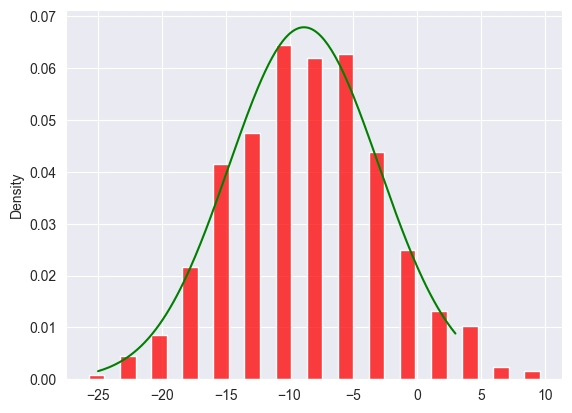
\includegraphics[width=\linewidth]{feelslikec1}
   \end{minipage} \hfill
\begin{minipage}{.48\textwidth}
     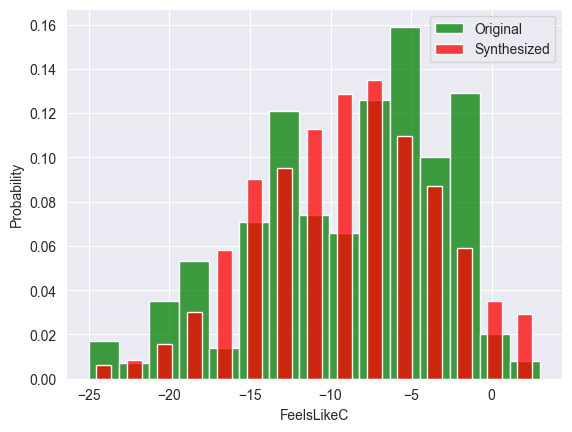
\includegraphics[width=\linewidth]{feelslikec}
   \end{minipage}
\caption{The histogram of the Box-Muller-generated sample vs the reference density and the histogram of observed FeelsLikeC.}
\label{fig: 7}
\end{figure}

As for the second sampling algorithm, we used ARS using Laplace standard distribution to simulate normal one. Two sample Kolmogorov-Smirnov test was performed under significance level $\widetilde{\alpha} = 0.05$. Its p-value$ \approx 4.4 \cdot 10^{-6}$ so it rejects the hypothesis that the synthesized sample came from the same distribution as our sample. Two figures in fig. \ref{fig: 8} demonstrate to what extent the generated sample is similar to the theoretical distribution and the empirical distribution of FeelsLikeC.


\begin{figure}[!h]
   \begin{minipage}{.48\textwidth}
     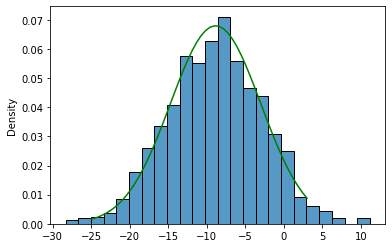
\includegraphics[width=\linewidth]{feelslikec3}
   \end{minipage} \hfill
\begin{minipage}{.48\textwidth}
     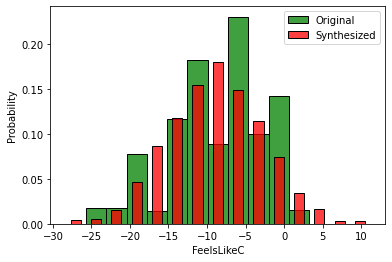
\includegraphics[width=\linewidth]{feelslikec2}
   \end{minipage}
\caption{The histogram of the ARS-generated sample vs the reference density and the histogram of observed FeelsLikeC.} 
\label{fig: 8}
\end{figure}

\subsection*{windspeedKmph}
In Lab \#1 it was obtained that the appropriate distribution for windspeedKmph is $Cauchy(loc, scale)$ with $loc \approx 11.637,\ scale \approx 2.830$. The only correction here is that we modified the distribution so that it is restricted on the range of the variable (at least, its values are non-negative). To simulate this corrected distribution we used both inverse transform sampling (ITS) and ARS using uniform distribution.

As soon as a sample of 1000 elements was obtained from the found distribution by the ITS algorithm, two sample Kolmogorov-Smirnov test was performed under significance level $\widetilde{\alpha} = 0.05$. Its p-value$ \approx 0.001$ so it rejects the hypothesis that the synthesized sample came from the same distribution as our sample. Two figures in fig. \ref{fig: 9} demonstrate to what extent the generated sample is similar to the theoretical distribution and the empirical distribution of windspeedKmph.

\begin{figure}[!h]
   \begin{minipage}{.48\textwidth}
     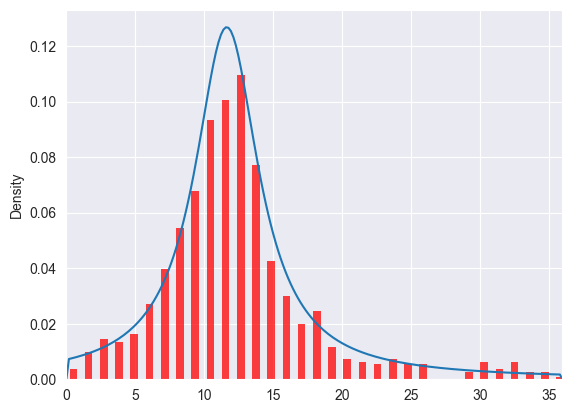
\includegraphics[width=\linewidth]{itsws1}
   \end{minipage} \hfill
\begin{minipage}{.48\textwidth}
     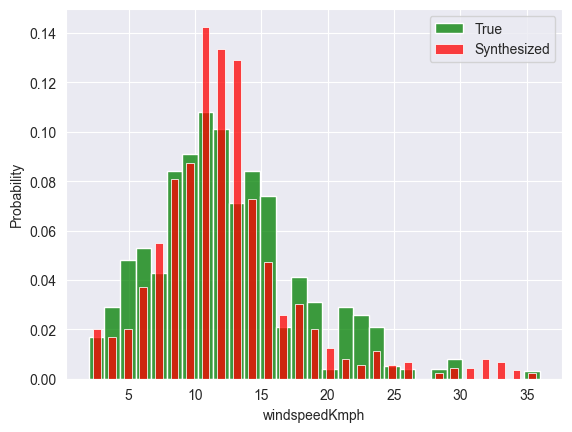
\includegraphics[width=\linewidth]{itsws}
   \end{minipage}
\caption{The histogram of the ITS-generated sample vs the reference density and the histogram of observed windspeedKmph.} 
\label{fig: 9}
\end{figure}

As for the second sampling algorithm, we used ARS using uniform distribution over the range of the variable to simulate normal one. Two sample Kolmogorov-Smirnov test was performed under significance level $\widetilde{\alpha} = 0.05$. Its p-value$ \approx 0.0004$ so it rejects the hypothesis that the synthesized sample came from the same distribution as our sample. Two figures in fig. \ref{fig: 10} demonstrate to what extent the generated sample is similar to the theoretical distribution and the empirical distribution of FeelsLikeC.


\begin{figure}[!h] 
   \begin{minipage}{.48\textwidth}
     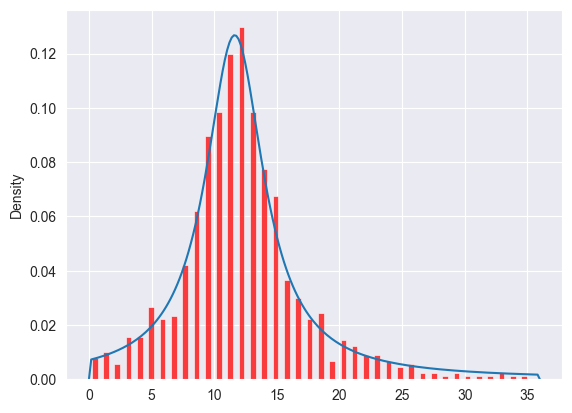
\includegraphics[width=\linewidth]{arsws1}
   \end{minipage} \hfill
\begin{minipage}{.48\textwidth}
     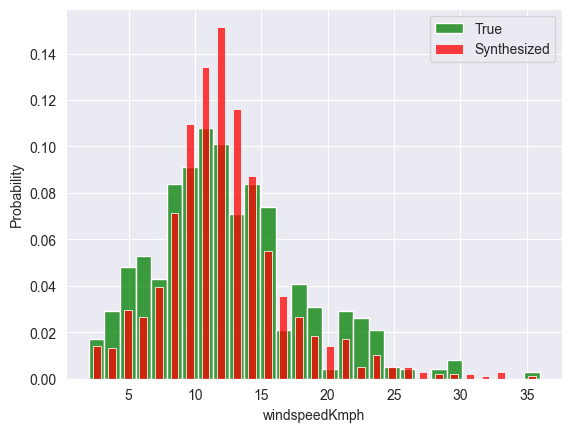
\includegraphics[width=\linewidth]{arsws}
   \end{minipage}
\caption{The histogram of the ARS-generated sample vs the reference density and the histogram of observed windspeedKmph.} 
\label{fig: 10}
\end{figure}



\section{Estimation of relations between predictors and chosen target variables}
In this section we study significance of relations between targets and chosen predictors. As was obtained in Lab \#2, variable State\_ is able to determine bimodality in the distribution of Friction\_mean so here we conclude that the former variable is worth using in our future study as a predictor.

As for other variables, we performed correlation analysis to find the variables among the predictors that significantly correlate with at least one target. The results of the correlation significance test for windspeedKmph, FeelsLikeC and Friction\_mean are provided in table \ref{tab: 1}, \ref{tab: 2} and \ref{tab: 3} correspondingly. As one can see, each of the predictors has significant correlation with at least one target. So we further use the variables moon\_illumination, Water\_mean, Height\_mean, pressure, State\_, totalSnow\_cm, humidity as predictors.


\begin{table}[!h]
\centering
\begin{tabular}{|l|r|r|r|r|}
\hline
windspeedKmph &   $\widehat{\rho}_n$  &      left &     right &        p-value \\
\hline
\cellcolor{blue!25} humidity          & 0.076246 &  0.014321 &  0.137589 &  1.588231e-02 \\
\hline
\cellcolor{blue!25} pressure          & -0.315770 & -0.370511 & -0.258844 &  1.366632e-24 \\
\hline
Height\_mean       & -0.033959 & -0.095751 &  0.028093 &  2.833401e-01 \\
\hline
\cellcolor{blue!25} totalSnow\_cm      & 0.314295 &  0.257316 &  0.369097 &  2.297680e-24 \\
\hline
Water\_mean        &  -0.030320 & -0.092140 &  0.031732 &  3.381442e-01 \\
\hline
\cellcolor{blue!25} moon\_illumination &  0.217900 &  0.158042 &  0.276163 &  3.264125e-12  \\
\hline
\end{tabular}
\caption{Correlation significance of  windspeedKmph vs predictors test results. Predictors highlighted by pale blue have significant correlation with the variable.}
\label{tab: 1}
\end{table}


\begin{table}[!h]
\centering
\begin{tabular}{|l|r|r|r|r|}
\hline
FeelsLikeC &   $\widehat{\rho}_n$  &      left &     right &        p-value \\
\hline
humidity          & 0.153972 &  0.092865 &  0.213923 &  9.974678e-07 \\
\hline
\cellcolor{blue!25} pressure          & -0.079740 & -0.141036 & -0.017835 &  1.165389e-02 \\
\hline
\cellcolor{blue!25} Height\_mean       & 0.122230 &  0.060697 &  0.182837 &  1.066483e-04 \\
\hline
 totalSnow\_cm      & 0.032002 & -0.030050 &  0.093809 &  3.120183e-01 \\
\hline
\cellcolor{blue!25} Water\_mean        & 0.397541 &  0.344027 &  0.448481 &  3.321284e-39 \\
\hline
\cellcolor{blue!25} moon\_illumination &  0.110915 &  0.049260 &  0.171727 &  4.415945e-04 \\
\hline
\end{tabular}
\caption{Correlation significance of FeelsLikeC vs predictors test results. Predictors highlighted by pale blue have significant correlation with the variable.}
\label{tab: 2}
\end{table}


\begin{table}[!h]
\centering
\begin{tabular}{|l|r|r|r|r|}
\hline
Friction\_mean &   $\widehat{\rho}_n$  &      left &     right &        p-value \\
\hline
humidity          & -0.027756 & -0.089595 &  0.034296 &   3.806060e-01 \\
\hline
\cellcolor{blue!25} pressure          & -0.281915 & -0.338001 & -0.223834 &   1.001731e-19 \\
\hline
\cellcolor{blue!25} Height\_mean       & -0.102377 & -0.163333 & -0.040642 &   1.187311e-03 \\
\hline
\cellcolor{blue!25} totalSnow\_cm      & -0.087782 & -0.148965 & -0.025930 &   5.472678e-03 \\
\hline
\cellcolor{blue!25} Water\_mean        &  0.071716 &  0.009767 &  0.133118 &   2.333191e-02 \\
\hline
\cellcolor{blue!25} moon\_illumination &  0.125759 &  0.064267 &  0.186300 &   6.671204e-05 \\
\hline
\end{tabular}
\caption{Correlation significance of Friction\_mean vs predictors test results. Predictors highlighted by pale blue have significant correlation with the variable.}
\label{tab: 3}
\end{table}

\section{Bayesian network}
To build and fit Bayesian networks (BN) in this lab we use BAMT toolkit \cite{bamt}. Firstly, we determined the types of targets and predictors. The variables State\_, FeelsLikeC and humidity are set to be discrete. The latter should be discrete since often humidity is measured in integers. The second has been set as discrete since the number of unique states of this variable is one of the lowest. The others are continuous.

\subsection{BN built on the multivariate analysis results}
By the usage of the multivariate analysis results provided in the tables \ref{tab: 1}, \ref{tab: 2} and \ref{tab: 3} and some physics reasoning, we have built BN which structure is presented in figure \ref{fig: 7}. The usage of the mixture of gaussian distributions is allowed. Since the built network has inner discrete nodes, logits are allowed.

\begin{figure}[!h]
\centering
   \begin{minipage}{0.7\textwidth}
     \includegraphics[width=\linewidth]{bn\_man}
   \end{minipage}
\caption{BN built on the correlation analysis results. Green nodes are MixtureGaussian, brown ones are Discrete, and green ones are ConditionalMixtureGaussian, pale pink ones are Logit and pink ones are ConditionalLogit}
\label{fig: 7}
\end{figure}

We performed sampling by means of the constructed BN (10000 synthetic observations) and then did two sample statistical tests, i.e. Kolmogorov-Smirnov and chi-square \cite{nist}, under significance level $\widetilde{\alpha}=0.05$.
\begin{outline}
\1 FeelsLikeC: chi-square test rejects the hypothesis that synthetic and original data came from the same distribution with p-value~$ \approx 0.00060$;
\1 windspeedKmph: Kolmogorov-Smirnov test rejects the analogous hypothesis with p-value~$ \approx 3\cdot 10^{-10}$;
\1 Friction\_mean: Kolmogorov-Smirnov test rejects the analogous hypothesis with p-value~$ \approx 1.2 \cdot 10^{-10}$.
\end{outline}

To be fair, the results are non-satisfactory so we hope that score-constructed BNs will provide good results. 

\subsection{BN built by score optimization and quality analysis}
We have built two BNs with gaussian mixtures allowed and logits denied by means of BIC and K2-score maximization. Their structures are provided in figures \ref{fig: 8} and \ref{fig: 9}.
To build the structure one needs to discretize the data.
\begin{figure}[!h]
\centering
   \begin{minipage}{0.7\textwidth}
     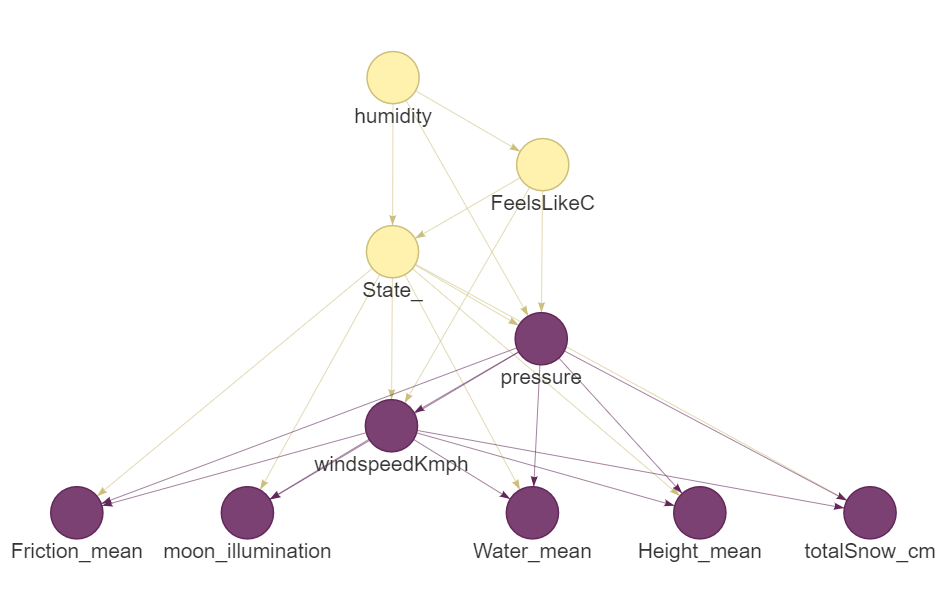
\includegraphics[width=\linewidth]{bn}
   \end{minipage}
\caption{BN built from BIC maximization. Orange nodes are Discrete, and blue ones are ConditionalMixtureGaussian}
\label{fig: 8}
\end{figure}

\begin{figure}[!h]
\centering
   \begin{minipage}{0.7\textwidth}
     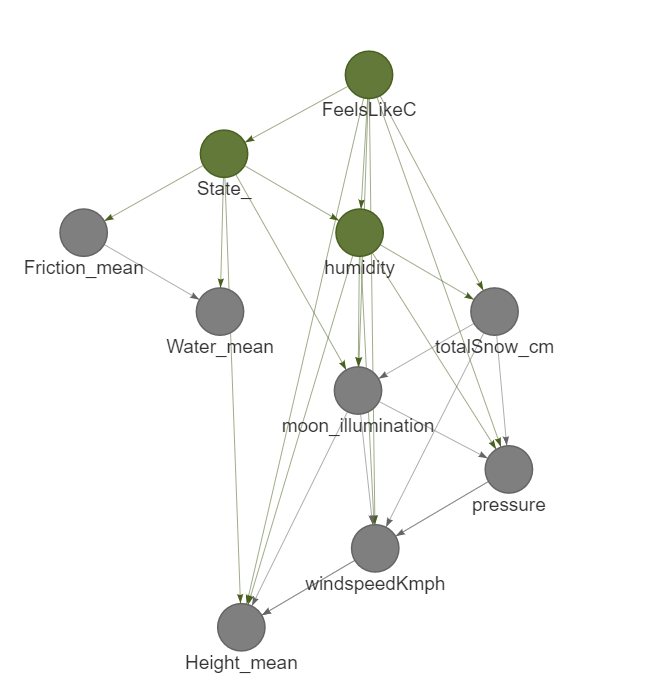
\includegraphics[width=\linewidth]{bn2}
   \end{minipage}
\caption{BN built from K2-score maximization. Green nodes are Discrete, and blue ones are ConditionalMixtureGaussian}
\label{fig: 9}
\end{figure}

As for the BN built on BIC, we sampled 10000 synthetic observations and performed the same tests. The results are as follows:
\begin{outline}
\1 FeelsLikeC: chi-square test failts to reject the hypothesis that synthetic and original data came from the same distribution with p-value~$\approx 0.915$;
\1 windspeedKmph: Kolmogorov-Smirnov test rejects the analogous hypothesis with p-value~$ \approx 8\cdot 10^{-6}$;
\1 Friction\_mean: Kolmogorov-Smirnov test rejects the analogous hypothesis with p-value~$ \approx 0.00047$.
\end{outline}

Then we did the same for the BN built on K2-score:
\begin{outline}
\1 FeelsLikeC: chi-square test failts to reject the hypothesis that synthetic and original data came from the same distribution with p-value~$ \approx 0.999$;
\1 windspeedKmph: Kolmogorov-Smirnov test rejects the analogous hypothesis with p-value~$\approx 0.0001$;
\1 Friction\_mean: Kolmogorov-Smirnov test fails to reject the analogous hypothesis with p-value~$ \approx 0.08$.
\end{outline}

As one can see, the second BN exhibits good quality of synthetic data. Histograms of the generated target variables are presented in figure \ref{fig: 10}

\begin{figure}[!h]
   \begin{minipage}{.48\textwidth}
     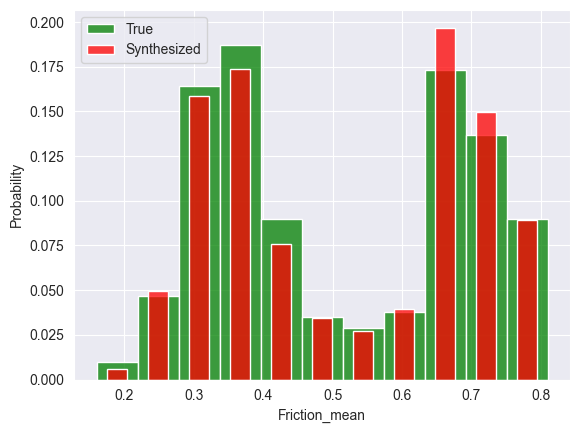
\includegraphics[width=\linewidth]{bn21}
   \end{minipage} \hfill
\begin{minipage}{.48\textwidth}
     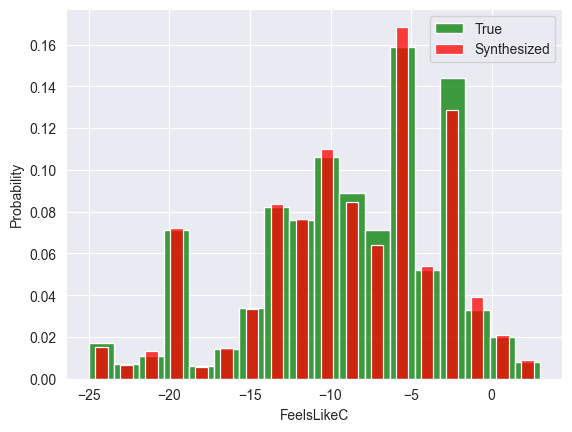
\includegraphics[width=\linewidth]{bn22}
   \end{minipage}\\
\centering
\begin{minipage}{.48\textwidth}
     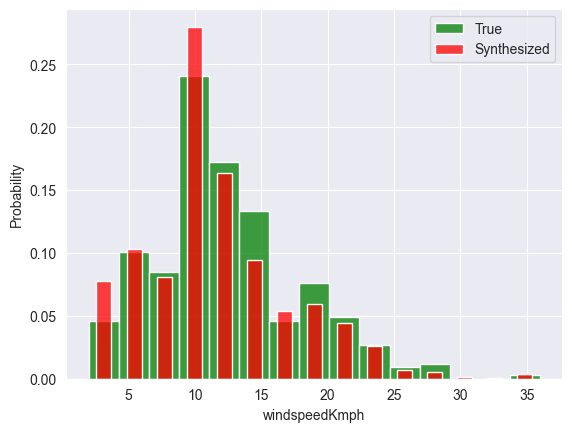
\includegraphics[width=\linewidth]{bn23}
   \end{minipage}
\caption{The histograms of targets: synthetic generated by BN based on K2-score vs original}
\label{fig: 10}
\end{figure}

Also we have checked the quality of synthetic data in the sense of missing data imputation. The experiment was conducted as follows: we obtained another subsample with 1000 observations from the original dataset and assign NA-value to the target variables of 400 randomly chosen individuals. Next, we have predicted missed target values given the evidence of predictors. Unfortunately, 236 observations were left with NA so we discard them from further consideration and the ones corresponding from the original subsample. At last, we compared original data and recovered one by means of statistical tests and analyzing of histograms. The results of tests are as follows:
\begin{outline}
\1 FeelsLikeC: chi-square test failts to reject the hypothesis that recovered and original data came from the same distribution with p-value~$ \approx 0.991$;
\1 Friction\_mean: Kolmogorov-Smirnov test fails to reject the analogous hypothesis with p-value~$ \approx 0.910$.
\end{outline}

The histograms are illustrated in figure \ref{fig: 11}.

\begin{figure}[!h]
   \begin{minipage}{.48\textwidth}
     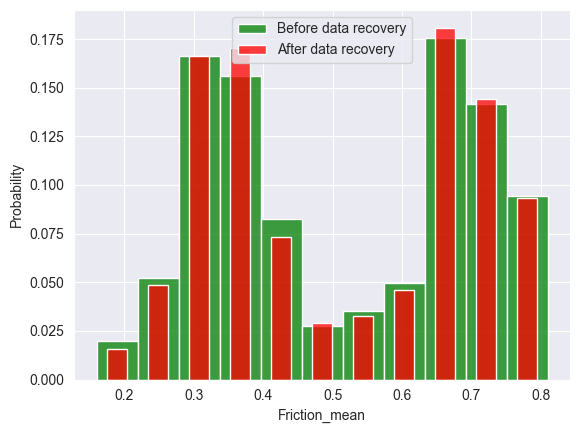
\includegraphics[width=\linewidth]{bn31}
   \end{minipage} \hfill
\begin{minipage}{.48\textwidth}
     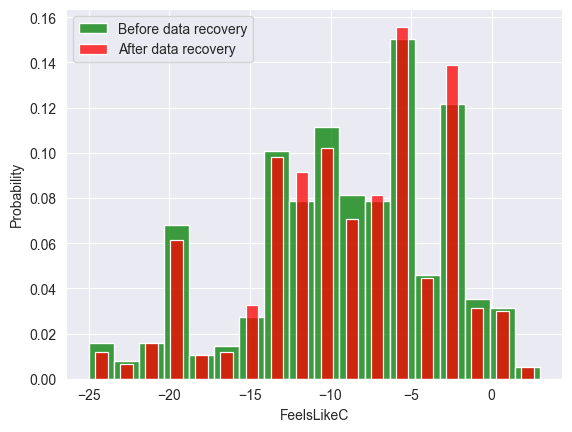
\includegraphics[width=\linewidth]{bn32}
   \end{minipage}\\
\caption{The histograms of targets: recovered by BN based on K2-score vs original}
\label{fig: 11}
\end{figure}

We may conclude that the built BN is worth using in missed data imputation.

\section{Appendix}
The Python notebook related to the aforementioned calculations is presented in Github \cite{repogithub}.

{\small \bibliography{biblio}}
\bibliographystyle{ugost2008s}

\end{document}